\documentclass[9pt,twocolumn,twoside]{gsag3jnl}

\articletype{inv} % article type

\usepackage{bm}
\usepackage{tabu}
\usepackage{graphicx}
\usepackage{caption}
\usepackage{subcaption}

\newcommand{\T}{^\text{T}}
\newcommand{\N}{\text{N}}
\newcommand{\twolinecell}[2][c]{%
  \begin{tabular}[#1]{@{}c@{}}#2\end{tabular}}
\graphicspath{{images/}}

\newcommand{\redstar}{\textcolor{red}{*}}


\title{\texttt{vqtl}: An \texttt{R} package for QTL Mapping on Phenotypes with Heterogeneous Variance}

\author[$\ast$]{Robert W. Corty}
\author[$\ast, 1$]{William Valdar}
\affil[$\ast$]{Department of Genetics, University of North Carolina at Chapel Hill}


\keywords{QTL mapping, variance heterogeneity}
\runningtitle{R package vqtl} % For use in the footer
\correspondingauthor{Robert Corty}
\setboolean{displaycopyright}{true}

\begin{abstract}
Existing methods for QTL mapping in experimental crosses assume that the amount of residual variation is constant across all individuals.
Many common situations can violate this assumption.
For example, female mice may have more variable phenotypes than males, some experimenters may make more precise measurements than others, and specific genetic loci may influence the extent of variation between individuals.
In all such cases, the heterogeneous variance modeling approach demonstrated here provides higher power, better protection against false positives, and allows for detection of QTL that influence phenotype variance, termed vQTL.
The \texttt{R} package \texttt{vqtl} makes it easy for geneticists to apply the heterogeneous variance model, control family-wide error rate (FWER), and visualize and interpret their results.
Because this package is interoperable with the popular \texttt{R/qtl} package and uses many of the same data structures and input patterns, it will be easy for geneticists to analyze the results of their experimental crosses with \texttt{vqtl}, possibly discovering new QTL.
Here, we demonstrate typical usage.
\end{abstract}

\begin{document}

\maketitle
\thispagestyle{firststyle}
\logomark
\articletypemark
\marginmark
\firstpagefootnote
\correspondingauthoraffiliation{Correspondence e-mail: william.valdar@unc.edu}
\vspace{-11pt}%

\noindent Experimental crosses of inbred organisms have been a cornerstone of forward genetics for over a century \citep{mendel1866}.
They have provided important insights on nearly every trait of interest in human disease, agriculture, and livestock production.
Studies across all these diverse fields were enabled by advances in methods for efficient breeding, phenotyping \citep{Yang2014a}, genotyping \citep{Williams1990}, statistical methods \citep{Lander1989a}, and software tools \citep{Broman2003}.

One assumption that has been constant throughout all these advances is that the extent of residual variation is constant across all organisms in a study population.
Said another way, it has always been assumed that no environmental factors and no genetic factors influence the extent of residual phenotype variation.
In the companion piece of this article, we introduced a statistical modeling approach that accommodates heterogeneity in residual variation within a study population.
We further demonstrated two critical benefits of using this ``simultaneous mean-variance'' modeling approach.

\begin{enumerate}
	\item It allows for the detection of genetic loci that influence residual phenotype variation, which are likely to play central roles in the network of molecular interactions that gives rise to a complex trait.
	\item It allows for accurate consideration of the quantity of information provided by each individual.  Individuals with less residual phenotype variance provide more information about the mean of the groups to which they belong, as is evident in the standard equation for the standard error of the mean: $\text{SE}_\mu = \sigma/\sqrt{n}$.
\end{enumerate}

The companion piece of this article is based on our reanalysis of an F2 intercross of two mouse strains carried out and published in 2008, but some of the results are completely novel.
In support of other researchers who may be interested in reanalysing previously-conducted mapping studies using the simultaneous mean-variance mapping approach, we have composed an R package that provides functions for conducting mean-variance genome scans, assessing the statistical significance of results, and visualizing and interpreting significant findings.
R package \texttt{vqtl} uses the same \texttt{cross} data structure as the popular \texttt{qtl} package and is available on \texttt{CRAN}, so it is easy to get started.

Here, we demonstrate typical usage of the \texttt{vqtl} package.
The code used to generate all statistics and figures in this paper is available at \texttt{github.com/rcorty}.


\section*{Simulated Experimental Cross}

We used \texttt{R/qtl} to simulate the experimental cross to be analyzed.
The simulated population consists of 200 male and 200 female F2 offspring, with 3 chromosomes of length 100 cM, each tagged by 30 equally-spaced markers and genotype probabilities estimated by HMM to 2 cM separation.
We simulate four phenotypes

\begin{enumerate}
	\item \texttt{phenotype1} consists only of random noise and will serve as an example of negative results for all tests
	\item \texttt{phenotype2} is influenced by the 15th marker on chromosome one.  The marker influences the mean of the phenotype, but not the variance, so it will serve as an example of a pure ``mQTL''.
	\item \texttt{phenotype3} is influenced by the 15th marker on chromosome two.  The marker influences the variance of the phenotype, but not the mean, so it will serve as an example of a pure ``vQTL''.
	\item \texttt{phenotype4} is influenced by the 15th marker on chromosome three.  The marker influences both the mean and the variance of the phenotype, so it will serve as an example of a joint ``mvQTL''.
\end{enumerate}

We additionally consider \texttt{phenotype1'} through \texttt{phenotype4'}, which have the same genetic effects as \texttt{phenotype1} through \texttt{phenotype4}, but additionally have covariate effects on phenotype variance.
All the same analyses and plots that are shown for \texttt{phenotype1} through \texttt{phenotype4} are shown for \texttt{phenotype1'} through \texttt{phenotype4'} in the supplementary materials.

\section*{Conducting a genome scan}

The central function for genetic mapping in package \texttt{qtl} is \texttt{scanone}.
Analogously, the central function for genetic mapping in package \texttt{vqtl} is \texttt{scanonevar}.

\texttt{scanonevar} takes three required inputs:

\begin{enumerate}
    \item \texttt{cross} contains the genetic and phenotypic information from an exerimental cross.  This object can be the same \texttt{cross} object used in package \texttt{qtl}.
    \item \texttt{mean.formula} specifies the phenotype to be mapped, the covariates to be corrected for, and the QTL terms to be fitted (\texttt{additive} and \texttt{dominance} components by default).  The \texttt{mean.formula} uses the standard \texttt{R} formula notation.
    \item \texttt{var.formula} specifies the covariates to be corrected for as well as the QTL terms to be fitted (\texttt{additive} and \texttt{dominance} components by default) in modeling the residual variance.  The \texttt{var.formula} also uses the standard \texttt{R} formula notation.
\end{enumerate}

Optional argument \texttt{chrs} is used to specify a subset of chromosomes to be scanned, defaulting to all chromosomes.
Optional argument \texttt{return.covar.effects} is used to specify whether or not fitted effects of all covariates should be returned as part of the scan result, defaulting to \texttt{FALSE}.

Unlike \texttt{scanone}, which only tests for association between each locus and the phenotype mean, \texttt{scanonevar} computes three tests for each locus -- association with phenotype mean, association with phenotype variance, and joint association with phenotype mean and variance.
The statistic for each of these associations is a LOD score, the log of the ratio of the likelihood of the alternative model to the null model.
The details of the null and alternative models used in each of the three tests can be found in the companion article.
LOD scores are hard to compare across autosomal and sex chromosomes due to the difference in number of parameters.
The $p$-value of each LOD score is also calculated, based on the asymptotic $\chi^2$ distribution with the appropriate degrees of freedom of each test, but the interpretation of these $p$-values is clouded by the multiplicity of tests that are conducted in each scan.
Assessing the significance of the LOD scores in a manner that controls family-wide error rate (FWER) to the desired level is decribed below and is the recommened method for assessing the significance of QTL mapping results.

The object returned by the \texttt{scanonevar} function has class \texttt{scanonevar}.
Calling \texttt{plot} on this object produces a publication-quality plot that shows the three association statistics at each locus.
Calling \texttt{summary} on this object produces a summary of how the scan was conducted and what the results were.


\begin{figure}
    \begin{subfigure}{0.5\textwidth}
        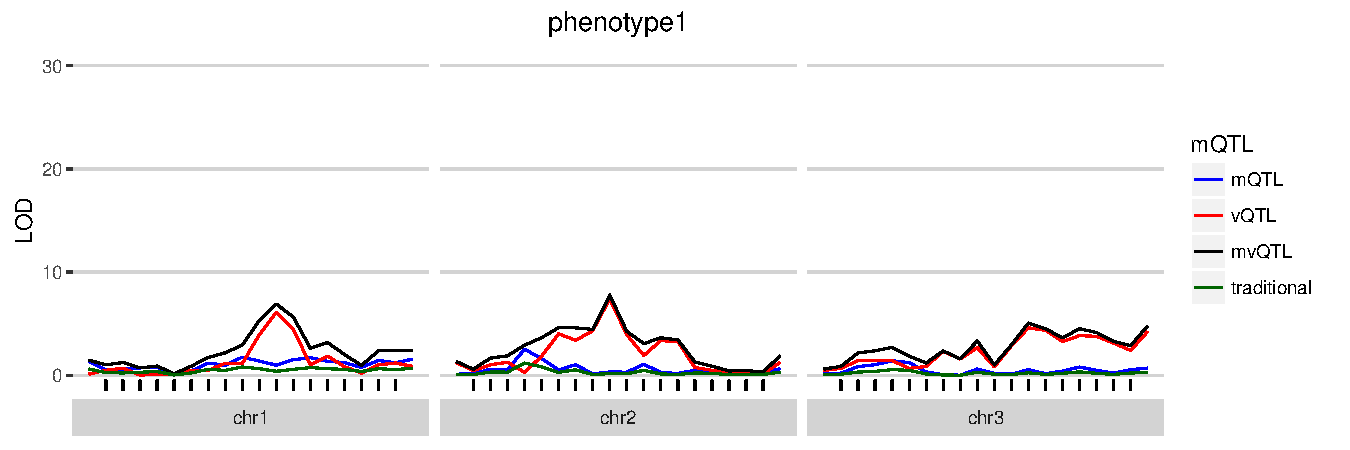
\includegraphics[width=\textwidth]{images/LOD_scan_phen1.pdf}
    \end{subfigure}

    \begin{subfigure}[b]{0.5\textwidth}
        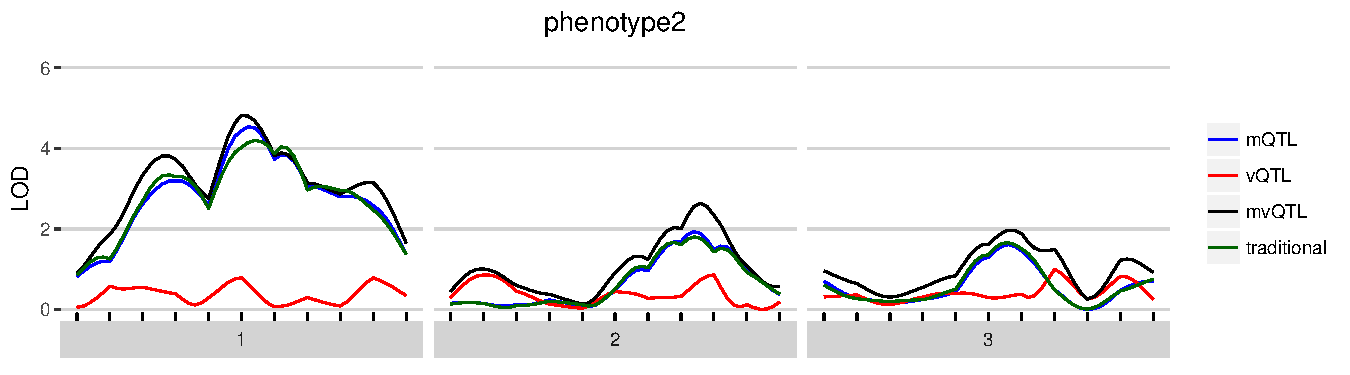
\includegraphics[width=\textwidth]{images/LOD_scan_phen2.pdf}
    \end{subfigure}

    \begin{subfigure}[b]{0.5\textwidth}
        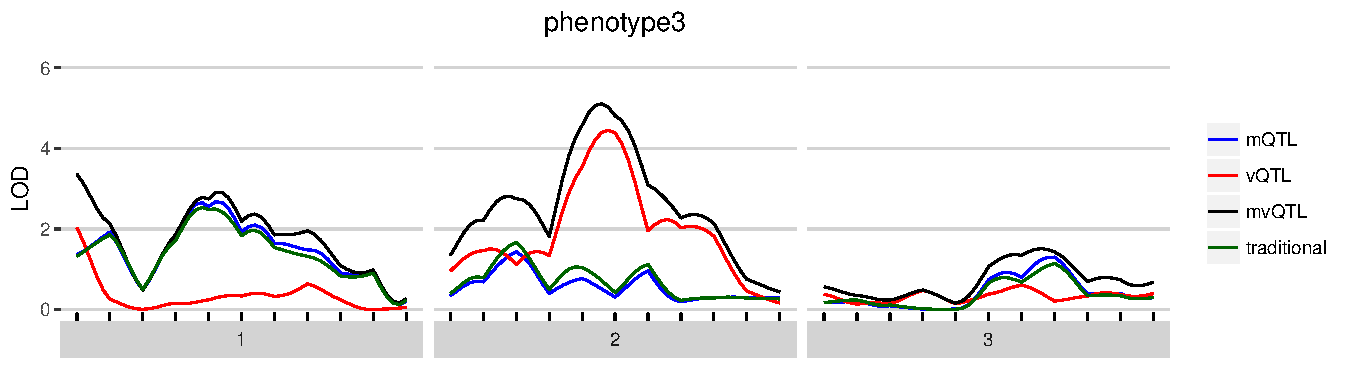
\includegraphics[width=\textwidth]{images/LOD_scan_phen3.pdf}
    \end{subfigure}
    
    \begin{subfigure}[b]{0.5\textwidth}
        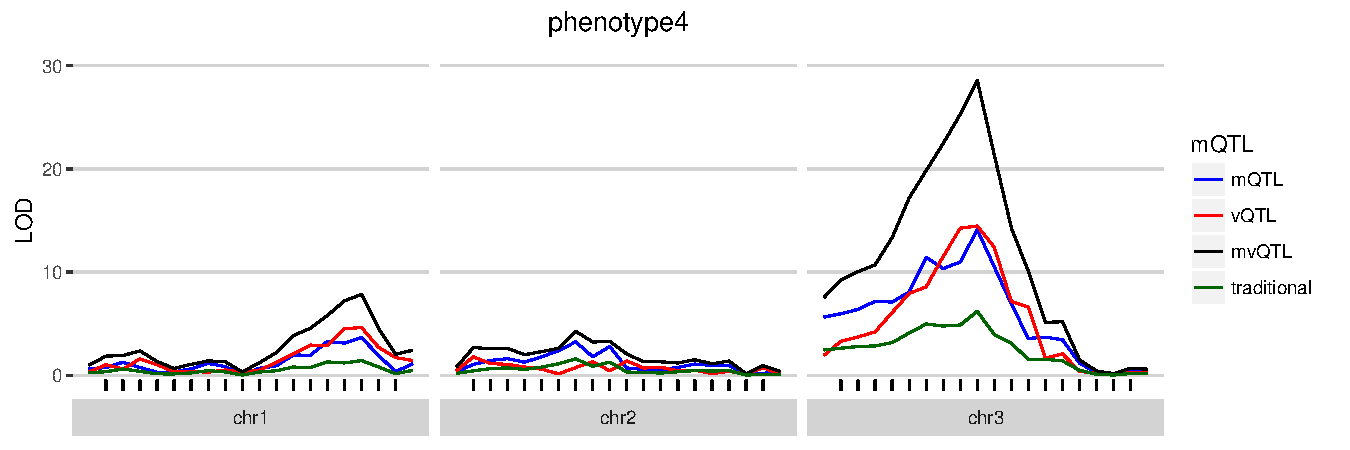
\includegraphics[width=\textwidth]{images/LOD_scan_phen4.pdf}
    \end{subfigure}
    
    \caption{For each of the four simulated phenotypes, we have the three new tests in black, blue, and red.  The traditional test is in green and clearly similar to the blue test in the vast manority of loci. \label{fig:lod_score_scans}}
\end{figure}



\section*{Assessing the Significance of Results}

The effective number of statistical tests conducted in a family of tests (a genome scan) is typically must be estimated to control family-wide error rate (FWER).
The effective number of tests in a genome scan, however, is difficult to estimate.
One lower bound is the number of chromosomes.
Due to the randomization in meiosis no two non-syntenic loci are correlated in an experimental cross and therefore tests on different chromosomes are always independent.
But there are many tests conducted on each chromosome, so the number of chromosomes is an under-estimate.
One upper bound on the effective number of tests is the total number of loci.
But, loci on the same chromosome are often in linkage disequilibrium and so the total number of loci is an over-estimate.

Our empirical approach avoids the need to estimate the effective number of tests.
We conduct many genomes scans, each with its own permutation of the genotype probabilities and estimate an extreme value distribution for the genome-wide maximum LOD score of each test.
This approach is implemented in \texttt{scanonevar.perm}.

\texttt{scanonevar.perm} takes two required inputs:

\begin{enumerate}
	\item \texttt{sov} is the \texttt{scanonevar} object, the statistical significance of which will be assessed.
	\item \texttt{n.perms} is the number of permutations to conduct.
\end{enumerate}

The object returned by \texttt{scanonevar.perm} is a \texttt{scanonevar} object with one important additional piece of information.
An empirical $p$-value for each test at each locus is included.
These $p$-values are FWER-corrected, so a value of $0.05$ for a specific test at a specific locus implies that in 5\% of similar experiments where there is no true genotype-phenotype association, we would expect to observe \textit{some} locus this significant or more significant.
A list of the per-genome-scan maximum observed LOD for each test and each chromosome type.


Accurate estimation of the FWER-controlled $p$-values requires many permutation scans.
We recommend at least 100, and rarely more than 1000.
These permutation scans can be broken into groups, run on separate computers, and combined with the generic \texttt{c} function.

\begin{figure}
    \begin{subfigure}{0.5\textwidth}
        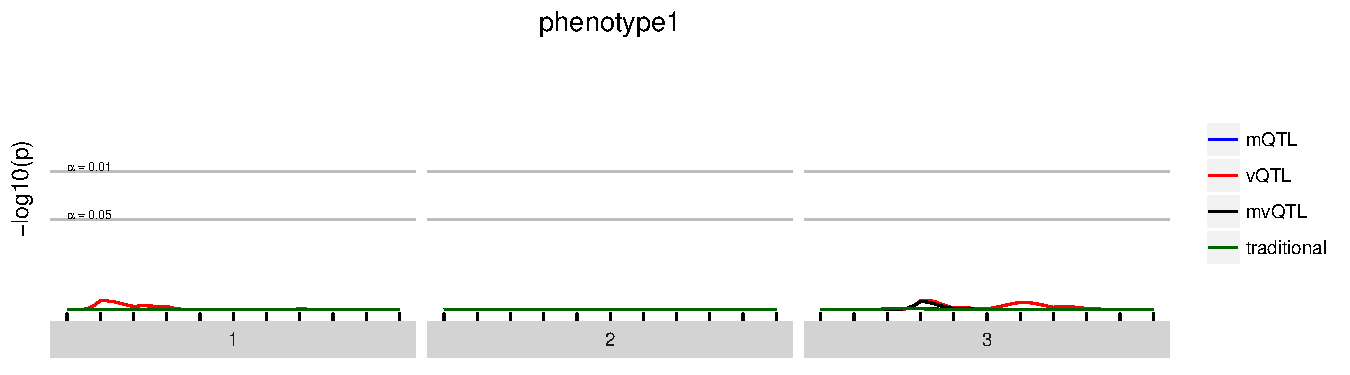
\includegraphics[width=\textwidth]{images/empir_p_scan_phen1.pdf}
    \end{subfigure}

    \begin{subfigure}[b]{0.5\textwidth}
        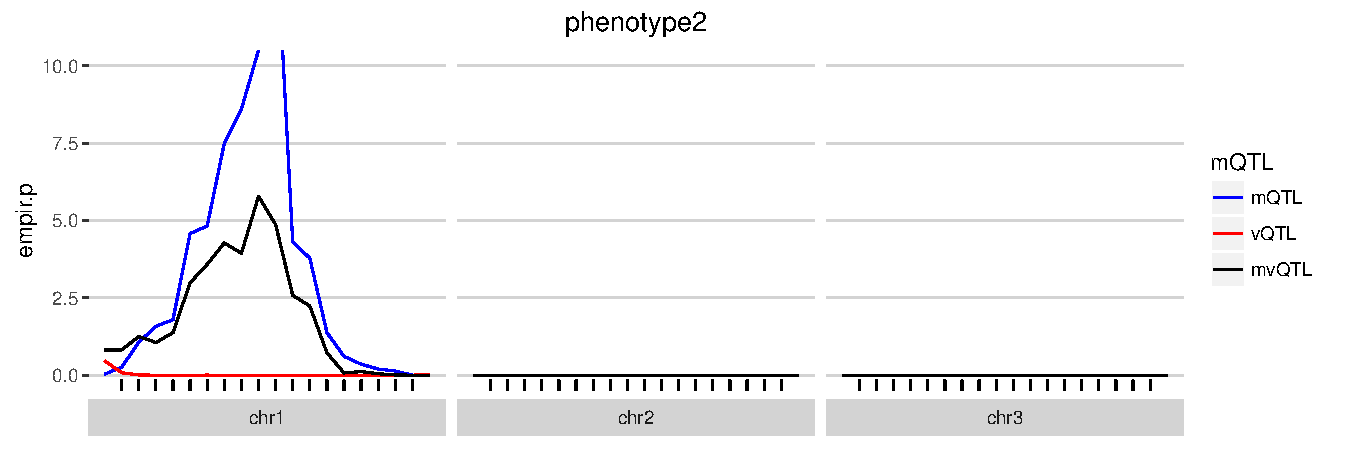
\includegraphics[width=\textwidth]{images/empir_p_scan_phen2.pdf}
    \end{subfigure}

    \begin{subfigure}[b]{0.5\textwidth}
        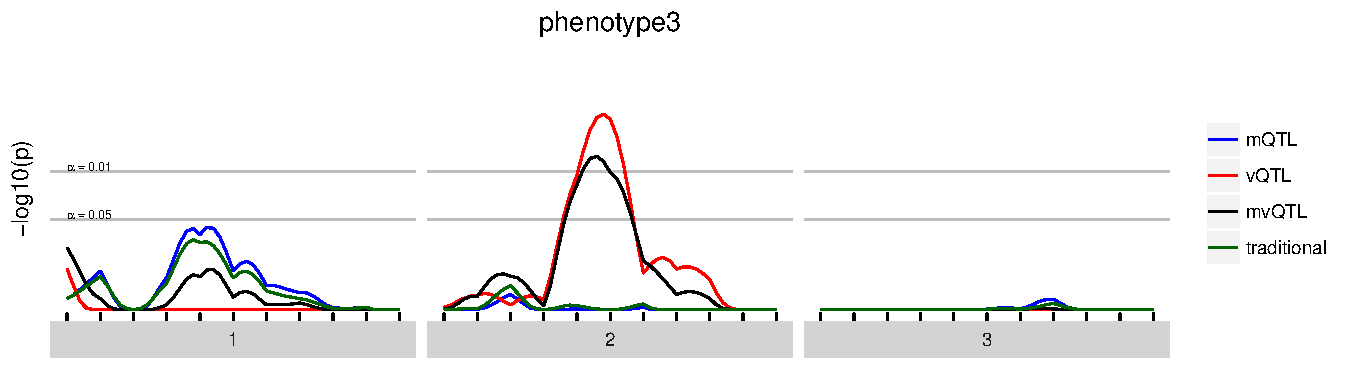
\includegraphics[width=\textwidth]{images/empir_p_scan_phen3.pdf}
    \end{subfigure}
    
    \begin{subfigure}[b]{0.5\textwidth}
        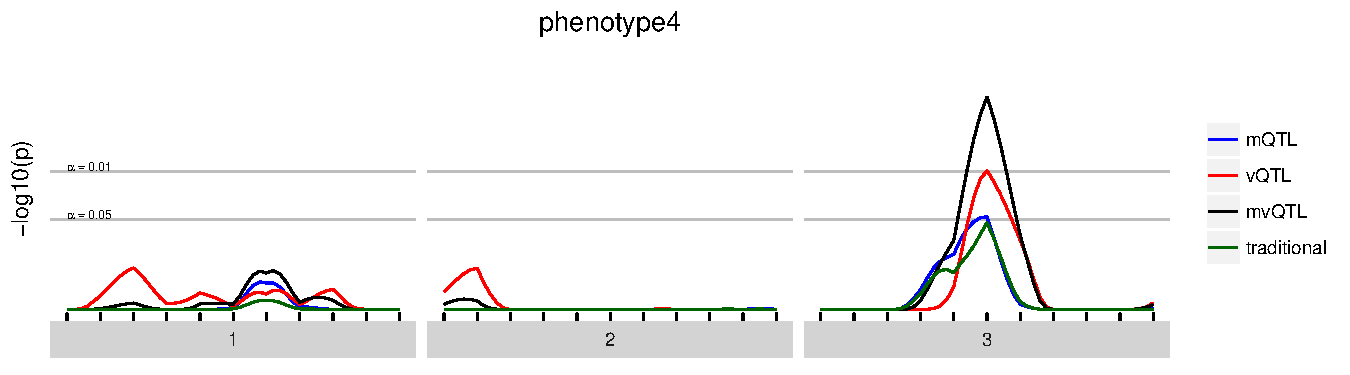
\includegraphics[width=\textwidth]{images/empir_p_scan_phen4.pdf}
    \end{subfigure}
    
    \caption{For each of the four simulated phenotypes, we have the three new tests in black, blue, and red.  The traditional test is in green and clearly similar to the blue test in the vast manority of loci. \label{fig:empir_p_scans}}
\end{figure}


% Figure~\ref{fig:lod_score_scans} shows the log of the odds at each locus for each of the four tests as a measure of association.
% This measure is traditional in QTL mapping, but in this scenario where multiple different tests are conducted at each locus, it suggesets a misleading interpretation, that points of different colors with the same LOD score represent an equal quantity of evidence against the null (no genetic effect).
% In fact, as is visible in the top panel of figure~\ref{fig:lod_score_scans}, the LOD score that results from differnet tests is different under the null.
% For example, the LOD score of the DGLM-joint test is always higher than the other three tests because all the other tests are ``nested'' inside the DGLM joint test.
% To put the four tests on a level playing field, we must conduct randomized genome scans and assess the observed LOD scores in the context of the per-scan maxima from the randomized genome scans, as illustrated in figure~\ref{fig:FWER}.


% \begin{figure}
% 	\includegraphics[width=0.5\textwidth]{images/FWER.pdf}
% 	\caption{Illustration of the method for controlling family-wide error rate in the genome scan. \label{fig:FWER}}
% \end{figure}



\section*{Investigate Significant Findings}




\bibliography{10_Aim1-2016_G3_PackageVQTL}

\end{document}